% Preamble
\documentclass[a4paper, 12pt]{article}
\usepackage[margin=1in]{geometry} % Set margin
\usepackage{pdfpages} % Insert pdf pages
\usepackage{amssymb,amsmath,amsthm, amsfonts} % Math libraries

% Custom commands
\newcommand{\sub}[1]{\subsection{\underline{#1}}}
\newcommand{\subsub}[1]{\subsubsection{\underline{#1}}}
\newcommand{\R}{\ensuremath{\mathbb{R}}}
\newcommand{\F}{\ensuremath{\mathbb{F}}}
\newcommand{\N}{\ensuremath{\mathbb{N}}}
\newcommand{\Onef}{\ensuremath{1_{\F}}}
\newcommand{\Zerof}{\ensuremath{0_{\F}}}
\newcommand{\eqbcuz}[1]{\text{~$\stackrel{(#1)}{=}$~}}
\newcommand{\eq}[1]{\begin{align*}#1\end{align*}}
\newcommand{\eqn}[1]{\begin{align}#1\end{align}}
\newcommand{\set}[1]{\big{\{} #1 \big{\}}}
\newcommand{\bigset}[1]{\bigg{\{} #1 \bigg{\}}}
\renewcommand{\qed}{\hfill\(\qedsymbol\)}
\newtheorem{lemma}{Lemma}

% Begin Document %
\begin{document}

% Title Page
\begin{titlepage}
    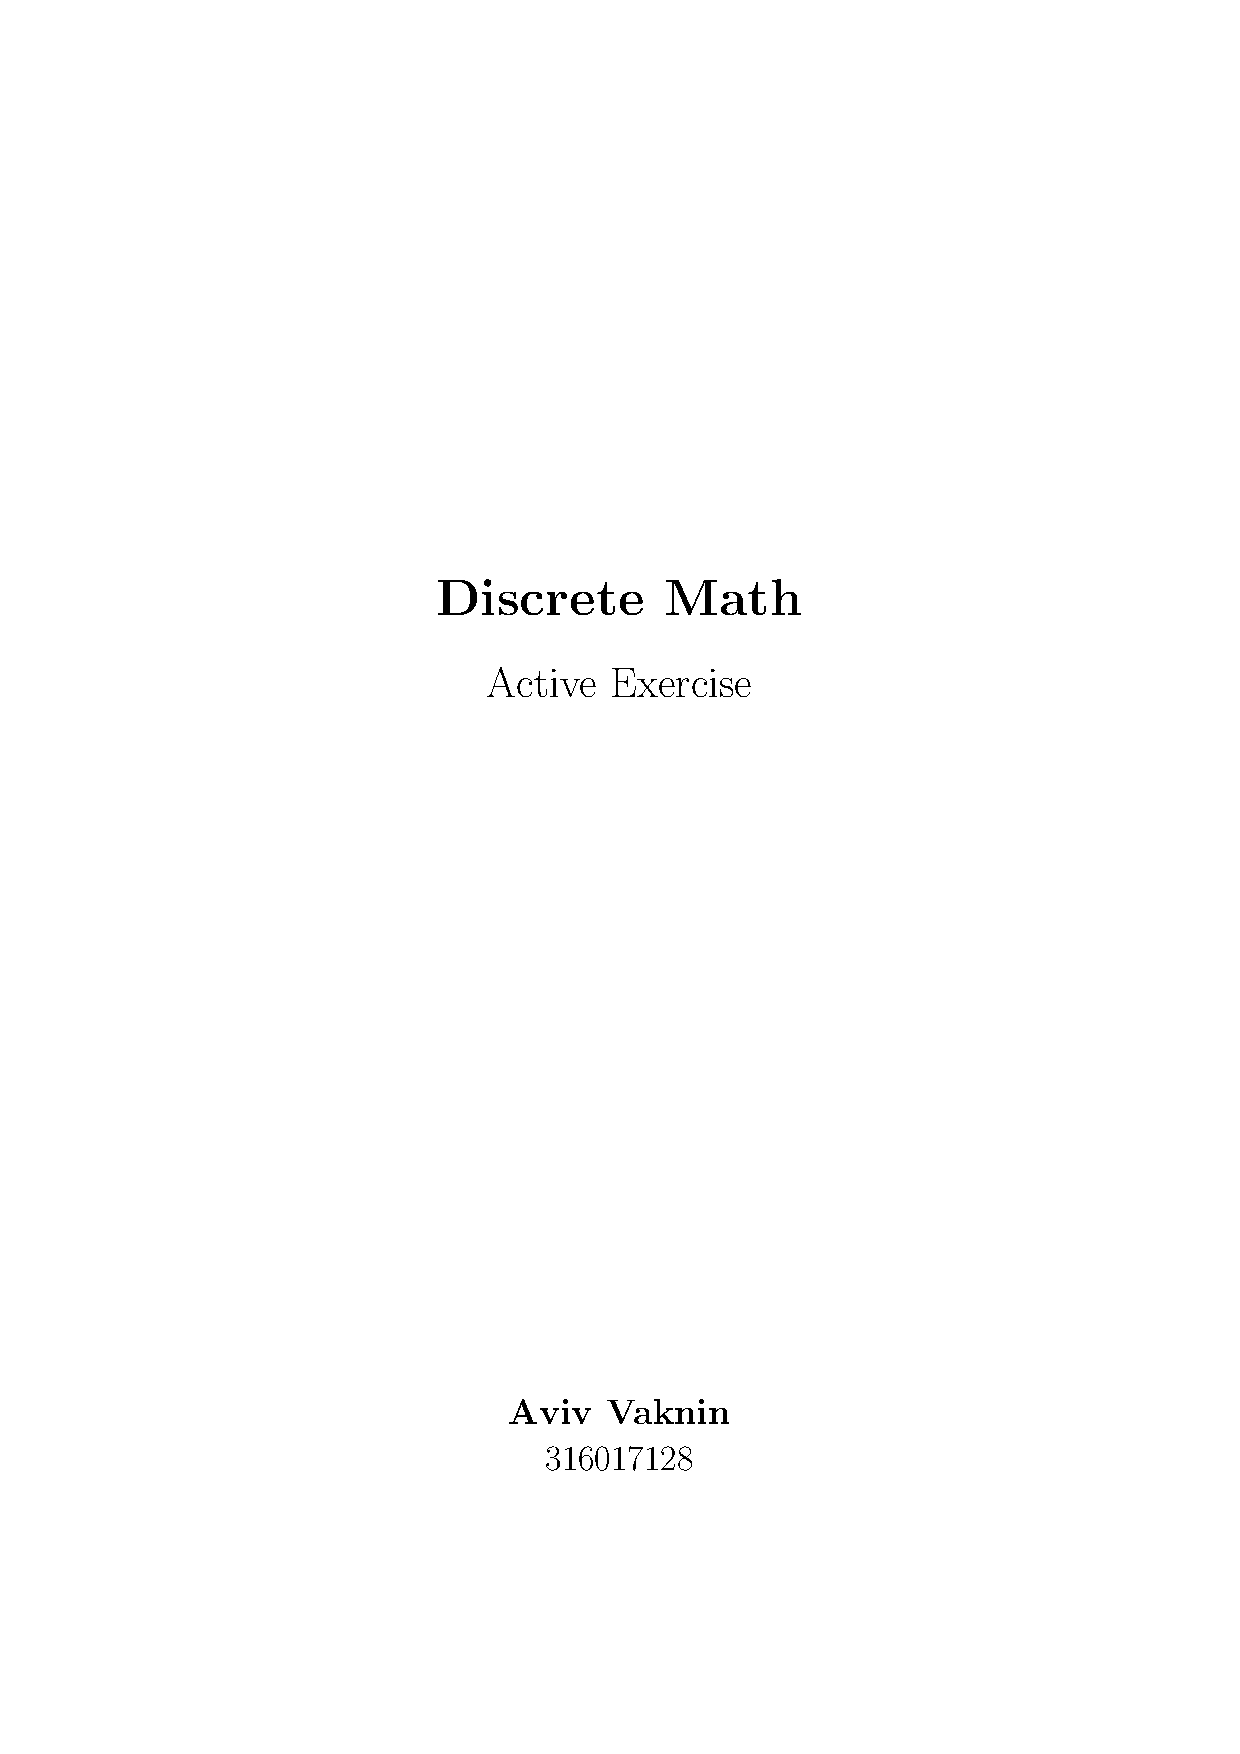
\includepdf{title.pdf}
\end{titlepage}

% 1
\section{Create an injective and surjective function from $\N$ to the natural numbers that can be divided by 5}
We'll define:
\eq{
    &f:N\longrightarrow{M}\\
    &f(n)=5n
}
We'll define $f$'s inverse function:
\eq{
    &f^{-1}:M\longrightarrow{N}\\
    &f^{-1}(n)=\frac{n}{5}
}
Now, we need to show that $f$ is injective and surjective.\\
We'll do that by showing that:
\eq{
    &f\circ{f^{-1}}=id_M\\
    &f^{-1}\circ{f}=id_N
}
\eq{
    &f\circ{f^{-1}}(n)=f(f^{-1}(n))=f(\frac{n}{5})=5\cdot\frac{n}{5}=n\\
    &f^{-1}\circ{f}(n)=f^{-1}(f(n))=f^{-1}(5n)=\frac{5n}{5}=n
}
Therefore, we've shown that:
\eq{
    &f\circ{f^{-1}}=id_M\\
    &f^{-1}\circ{f}=id_N
}
\qed

% 2
\section{Create a bijective function from $\N$ to $\N\times\set{1,2,3}$}
\eq{
    F(n)=\bigg{\{
        \begin{matrix}
            (\frac{n}{3},3)~~& 3|n\\
            (\frac{n+1}{3},2)~~& 3|n+1\\
            (\frac{n+2}{3},1)~~& 3|n+2
        \end{matrix}
    }
}
I am not sure how to prove this is bijective, but we can easily see that it is bijective,\\
as for every different $n\in\N$ a different ordered-pair will return.
\qed\pagebreak

% 3
\section{Prove that the following sets are not countable}
\sub{}
Let's look at:
\eq{
    B=\bigset{a+b\sqrt{2}:~a,b\in{Z}}
}
We can see that it includes all of the integers($\mathbb{Z}$) and some multiplicitive variations of $\sqrt{2}$.\\
Therefore, we can create a bijective function $F$ such that:
\eq{
    F: \N\longrightarrow{B}
}
Hence, \textit{B} is countable.\\
Therefore, if we deduct a countable set from a non-countable set, the result will be necessarily a non-countable set.
\sub{}
$\set{0,1}^{\N}$ is not countable, because it is a set of all of infinite sequences, as shown in lecture.\\
In the given set - B, there is no difference, as $f^{-1}({0})$ and $f^{-1}({1})$ are infinite, and that means that there are infinite sequences.

% 4
\section{Are the following sets countable?}
\sub{}
A is not countable because we can still create an infinite number of sequences of $\set{0,1}$.
\sub{}
A is countable because it can be viewed as a countable union on a countable number of finite sets.\\
As we've seen in the lecture, this type of union result in a countable set.

% 5
\section{Build a bijective function from (0,2) to (0,1)$\cup$(2,3)}
\eq{
    F(n)=\bigg{\{
        \begin{matrix}
            n && 0<n<1\\
            n+1 && 1<n<2\\
        \end{matrix}
    }
}
\pagebreak

% 6
\section{Build a bijective $f: A\longrightarrow{B}$ or prove that it cannot exist}
This function cannot exist.\\
It seems like B is "twice" as "big" as A.\\
For example, we can take $1\longrightarrow(1,0)$, and $-1\longrightarrow(-1,0)$.\\
However, that only fills half of the tuples of B.\\
This way, we'll only be able to build an injective function that will do it, but it will \textbf{not} be bijective.

\end{document}